\documentclass[17pt,xcolor=dvipsnames,table,dvipdfmx]{beamer}

\usepackage{slide}
\usepackage{appendixnumberbeamer}

\usepackage{math_macros}

\usepackage{import}
\usepackage{url}
\usepackage{diagbox}
\usepackage{array,colortbl}
\usepackage{hyperref}
% \hypersetup{
%     colorlinks=true,
%     citebordercolor=blue,
%     linkbordercolor=blue,
%     urlbordercolor=blue,
%     %citecolor=black,
% }
\usepackage{nicematrix}

\usepackage{booktabs}

\newcommand{\comment}[2]{\textcolor{green!35!black}{#1 \fbox{\scalebox{0.4}{#2}}}}

% 引用
\usepackage[backend=bibtex, sorting=none]{biblatex}
\addbibresource{./references.bib}
% 脚注に引用文献の情報を強引に乗せる
\newcommand*{\mycite}[1]{\parencite{#1} \citeauthor{#1} (\citeyear{#1})}
\renewcommand*{\footcite}[1]{\footnote{\mycite{#1}}}
\AtBeginBibliography{\scriptsize}

\title{MP3 (aka MPEG1-Layer3)}
\author[aikiriao]{aikiriao}
\date{2024.3.XX}


\begin{document}
\maketitle

\begin{frame}[c]
    \frametitle{あらすじ}
    % \tableofcontents[hideallsubsections]
    \tableofcontents
\end{frame}

\section{MP3概要}

\subsection{歴史}

\begin{frame}[c]
    \frametitle{歴史}
\end{frame}

\subsection{コーデック構造}

\begin{frame}[c]
    \frametitle{MP3のエンコーダ構造}
    \begin{figure}
        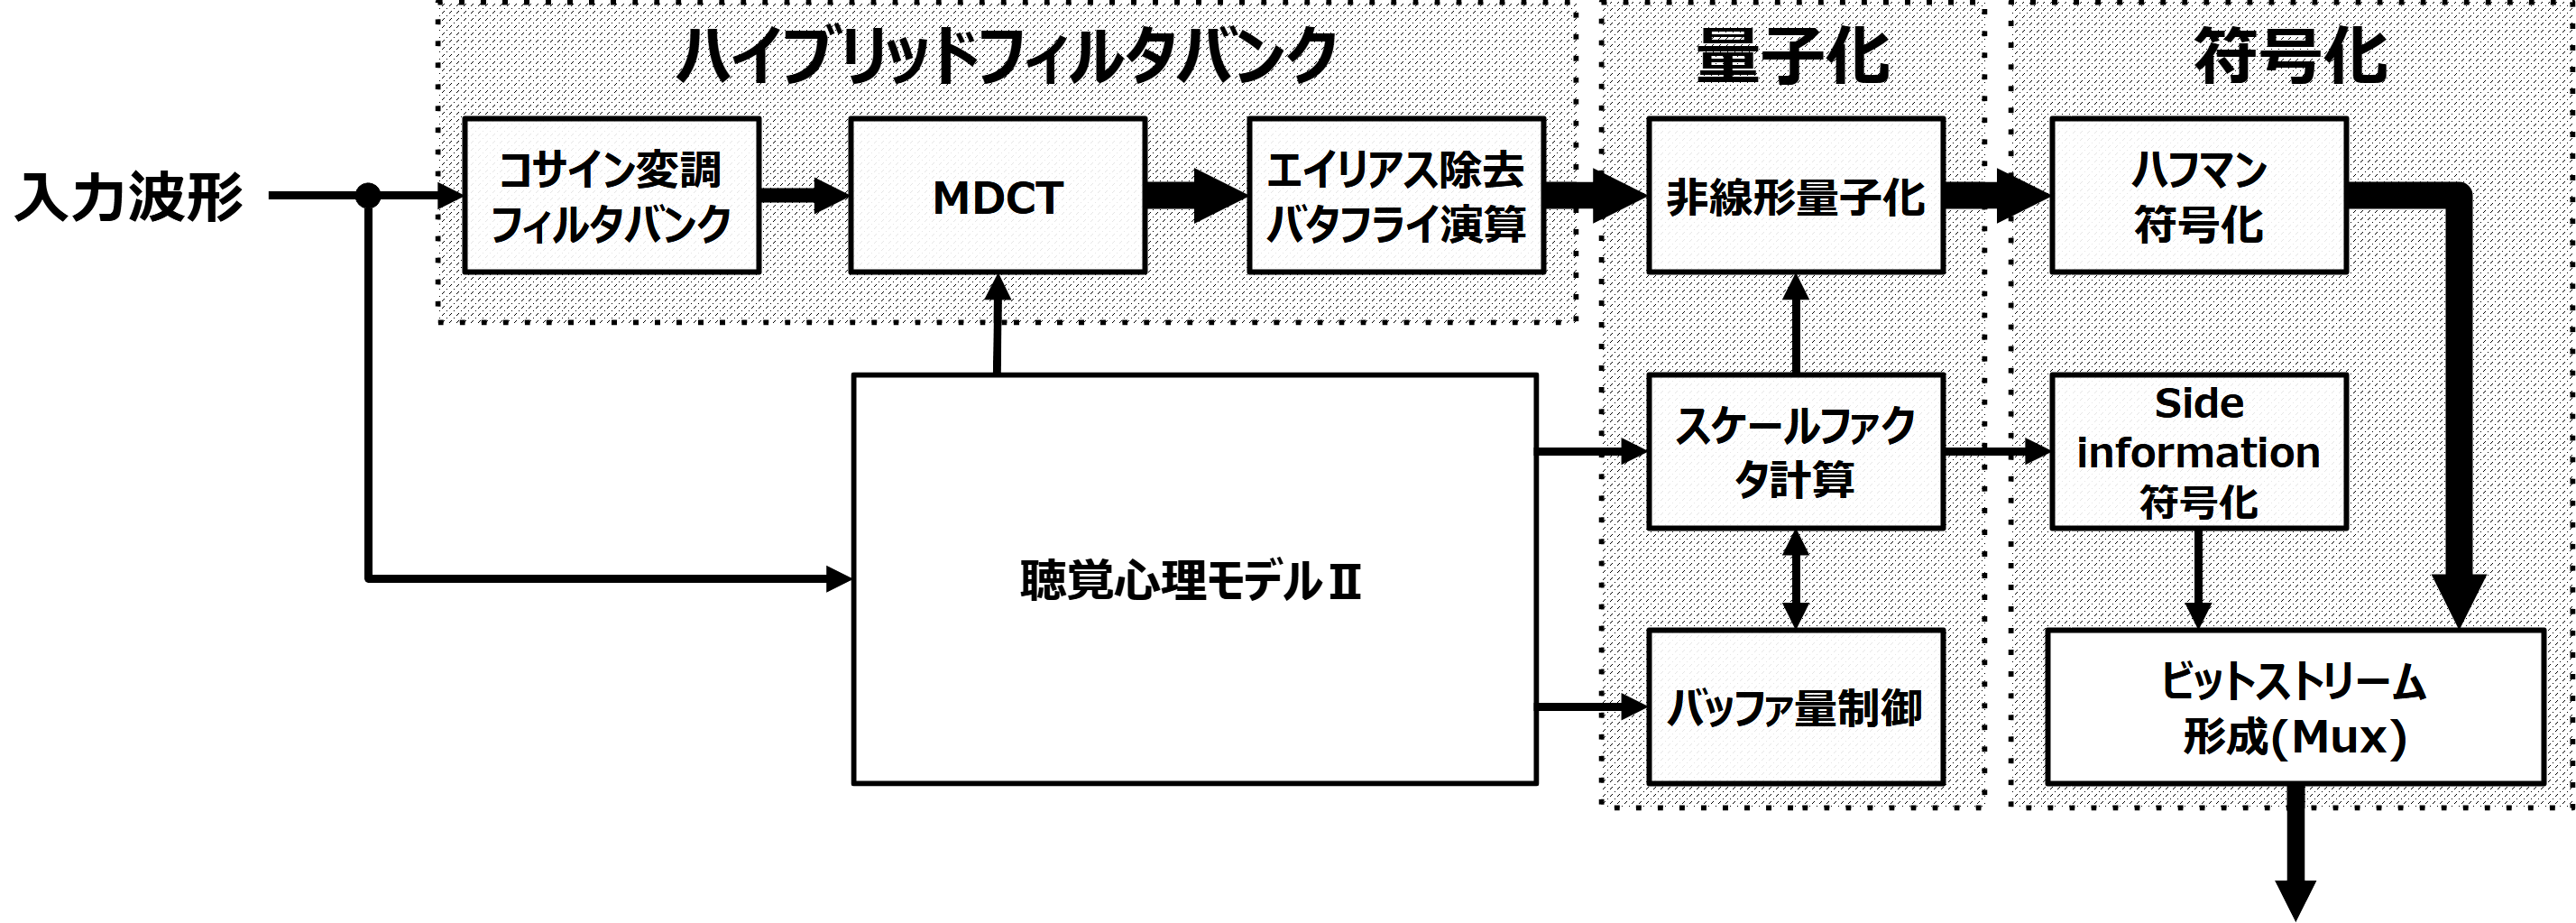
\includegraphics[width=115mm]{./figs/mp3_encoder_struct.png}
    \end{figure}
\end{frame}

\begin{frame}[c]
    \frametitle{MP3のデコーダ構造}
    \begin{figure}
        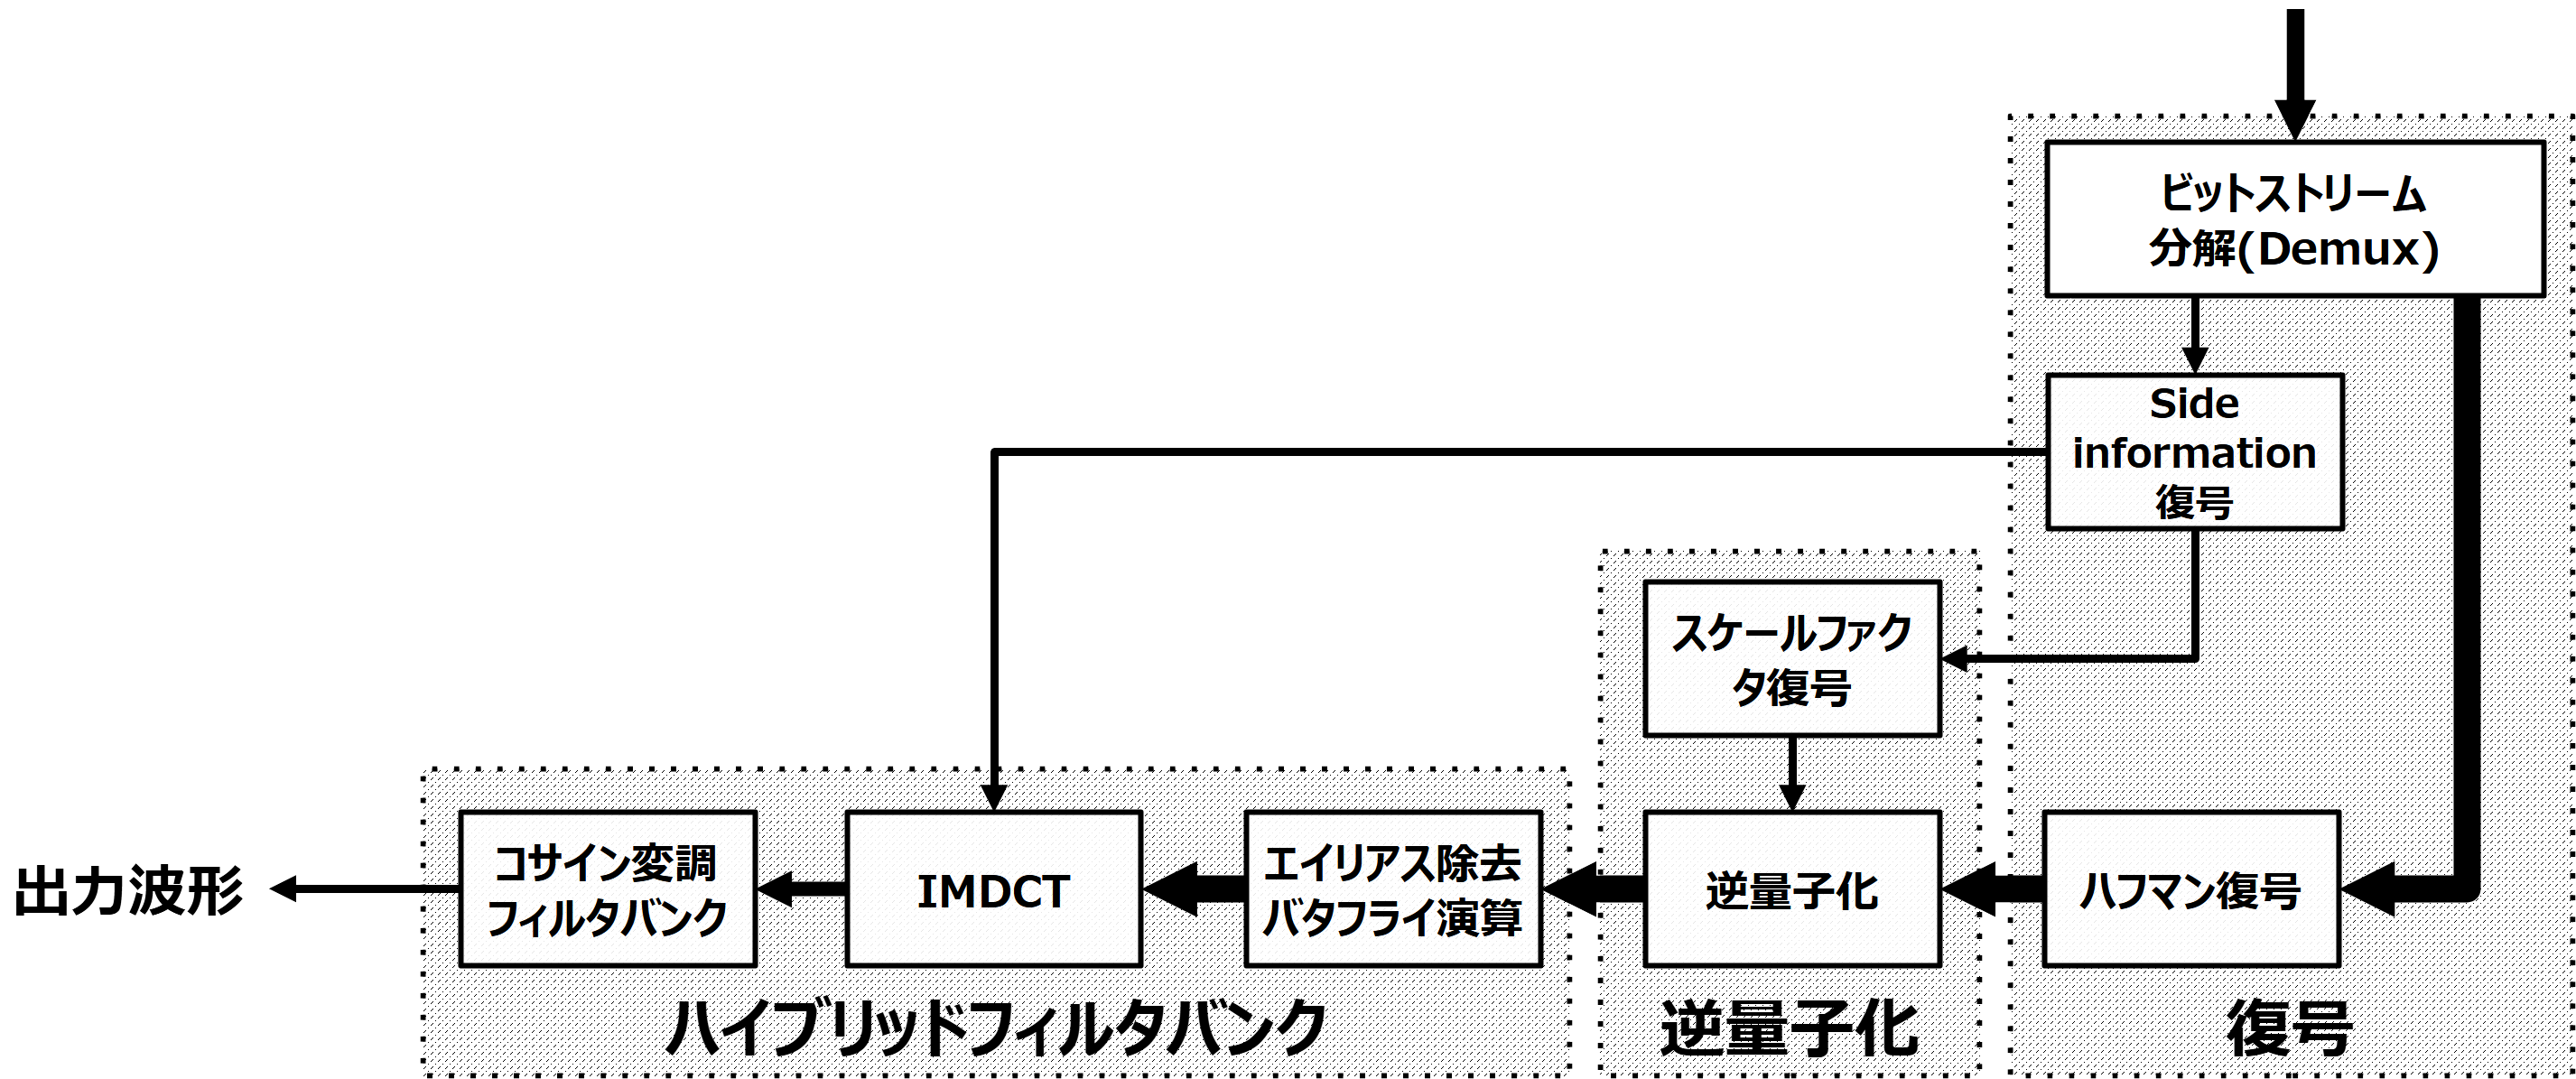
\includegraphics[width=115mm]{./figs/mp3_decoder_struct.png}
    \end{figure}
\end{frame}

\section{ハイブリッドフィルタバンク}

\subsection{コサイン変調フィルタバンク}

\begin{frame}[c]
    \frametitle{$M$分割フィルタバンク}
    \begin{figure}
        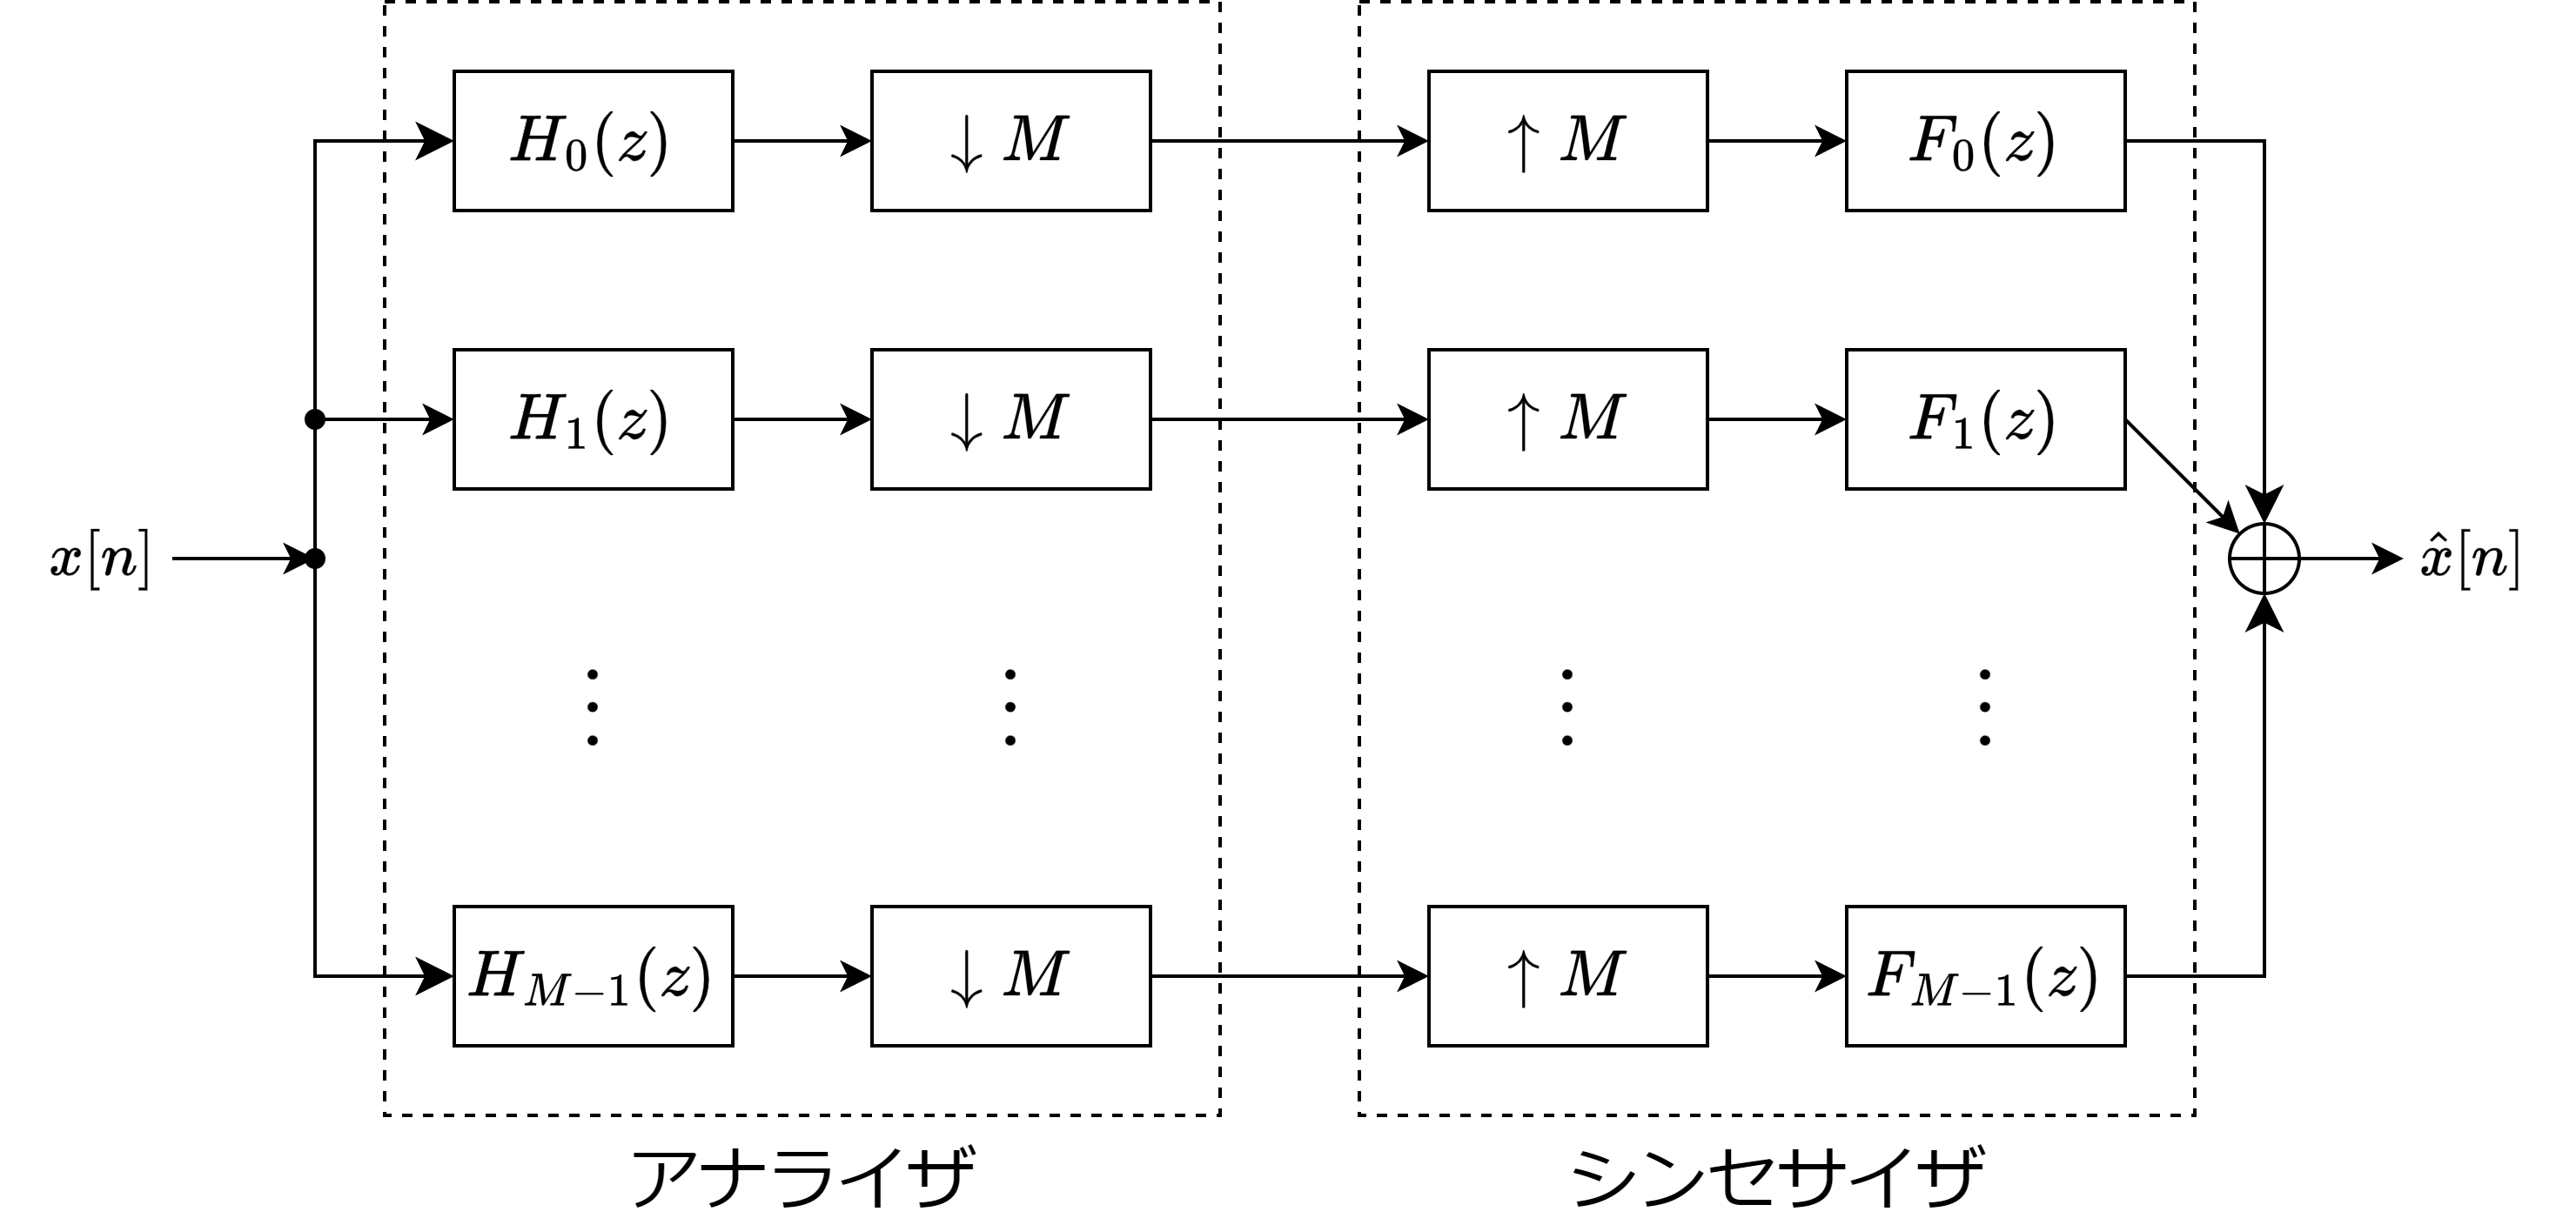
\includegraphics[width=120mm]{./figs/filter_bank.drawio.png}
    \end{figure}
\end{frame}

\begin{frame}[c]
    \frametitle{完全再構成}
    遅延・定数倍を除き入出力が一致すること:
    \begin{align}
        \hat{x}[n] = c x[n - n_{0}] \quad c \neq 0
    \end{align}
    $z$領域で,
    \begin{align}
        \hat{X}(z) = c z^{-n_{0}} X(z)
    \end{align}
    となること
    \begin{block}{}
        どんなどきに,$M$分割フィルタバンクが完全再構成になるか?
    \end{block}
\end{frame}

\begin{frame}[c]
    \frametitle{ポリフェーズ表現}
    フィルタ$H_{k}(z)\ (k = 0,...,M-1)$のインパルス応答を$h_{k}[n]$と書くとき,
    \scriptsize
    \begin{align*}
        H_{k}(z) &= \sum_{n = -\infty}^{\infty} h_{k}[n] z^{-n} = \sum_{n = -\infty}^{\infty} \sum_{l = 0}^{M - 1} h_{k}[nM + l] z^{-(nM+l)} \\
        &= \sum_{l = 0}^{M - 1} z^{-l} \sum_{n = -\infty}^{\infty}h_{k}[nM + l] z^{-nM} = \sum_{l = 0}^{M - 1} E_{k,l}(z^{M}) z^{-l}
    \end{align*}
    \normalsize
    \begin{block}{$h_{k}$の(タイプI)ポリフェーズ表現}
        \vspace{-13pt}
        \begin{align}
            E_{k,l}(z) = \sum_{n = -\infty}^{\infty} h_{k}[nM + l] z^{-n} \label{eq:type1_polyphase_representation}
        \end{align}
    \end{block}
\end{frame}

\begin{frame}[c]
    \frametitle{ポリフェーズ表現}
    $F_{k}(z)$のインパルス応答を$f_{k}[n]$と書くとき,
    \scriptsize
    \begin{align*}
        F_{k}(z) &= \sum_{n = -\infty}^{\infty} f_{k}[n] z^{-n} = \sum_{n = -\infty}^{\infty} \sum_{l = 0}^{M - 1} f_{k}[nM + l] z^{-(nM+l)} \\
        &= \sum_{n = -\infty}^{\infty} \sum_{l^{\prime} = 0}^{M - 1} f_{k}[nM + M - 1 - l^{\prime}] z^{-(nM + M - 1 - l^{\prime})} \\
        &= \sum_{l^{\prime} = 0}^{M - 1} z^{-(M - 1 - l^{\prime})} \sum_{n = -\infty}^{\infty} f_{k}[nM + M - 1 - l^{\prime}] z^{-nM} = \sum_{l^{\prime} = 0}^{M - 1} z^{-(M - 1 - l^{\prime})} R_{k,l}(z^{M})
    \end{align*}
    \normalsize
    \begin{block}{$f_{k}$の(タイプII)ポリフェーズ表現}
        \vspace{-13pt}
        \begin{align}
            R_{k,l}(z) = \sum_{n = -\infty}^{\infty} f_{k}[nM + M - 1 - l] z^{-n} \label{eq:type2_polyphase_representation}
        \end{align}
    \end{block}
\end{frame}

\begin{frame}[c]
    \frametitle{ポリフェーズ行列表現}
    \eqref{eq:type1_polyphase_representation}式を$l$について並べ,行列表現すると
    \scriptsize
    \begin{align*}
        \underbrace{\begin{bNiceMatrix}[margin, xdots/shorten=0.5em]
            H_{0}(z) \\
            H_{1}(z) \\
            \Vdots \\
            H_{M-1}(z)
        \end{bNiceMatrix}}_{\text{\normalsize $\ve{h}(z)$}}
        =
        \underbrace{\begin{bNiceMatrix}[margin, xdots/shorten=0.5em]
              E_{0,0}(z^{M}) &   E_{0,1}(z^{M}) & \Cdots &   E_{0,M-1}(z^{M}) \\
              E_{1,0}(z^{M}) &   E_{1,1}(z^{M}) & \Cdots &   E_{1,M-1}(z^{M}) \\
                      \Vdots &           \Vdots & \Ddots &            \Vdots  \\
            E_{M-1,0}(z^{M}) & E_{M-1,1}(z^{M}) & \Cdots & E_{M-1,M-1}(z^{M}) \\
        \end{bNiceMatrix}}_{\text{\normalsize $\ve{E}(z)$}}
        \underbrace{\begin{bNiceMatrix}[margin, xdots/shorten=0.5em]
                     1 \\
                z^{-1} \\
                \Vdots \\
            z^{-(M-1)}
        \end{bNiceMatrix}}_{\text{\normalsize $\ve{e}(z)$}}
    \end{align*}
    \normalsize
    \eqref{eq:type2_polyphase_representation}式も同様にして,以下のように書ける
    \scriptsize
    \begin{align*}
        \underbrace{\begin{bNiceMatrix}[margin, xdots/shorten=0.5em]
            F_{0}(z) \\
            F_{1}(z) \\
            \Vdots \\
            F_{M-1}(z)
        \end{bNiceMatrix}}_{\text{\normalsize $\ve{f}(z)$}}
        =
        \underbrace{\begin{bNiceMatrix}[margin, xdots/shorten=0.5em]
              R_{0,0}(z^{M}) &   R_{0,1}(z^{M}) & \Cdots &   R_{0,M-1}(z^{M}) \\
              R_{1,0}(z^{M}) &   R_{1,1}(z^{M}) & \Cdots &   R_{1,M-1}(z^{M}) \\
                      \Vdots &           \Vdots & \Ddots &            \Vdots  \\
            R_{M-1,0}(z^{M}) & R_{M-1,1}(z^{M}) & \Cdots & R_{M-1,M-1}(z^{M}) \\
        \end{bNiceMatrix}^{\mathsf{T}}}_{\text{\normalsize $\ve{R}(z)^{\mathsf{T}}$}}
        \underbrace{\begin{bNiceMatrix}[margin, xdots/shorten=0.5em]
            z^{-(M-1)} \\
          z^{-(M-1)+1} \\
                \Vdots \\
                     1
        \end{bNiceMatrix}}_{z^{-(M-1)}\ve{e}(z^{-1})}
    \end{align*}
\end{frame}

\begin{frame}[c]
    \frametitle{ポリフェーズ行列表現}
    $\tilde{\ve{e}}(z) = \ve{e}(z^{-1})^{\mathsf{T}}$とすると行列表現は
    \begin{align}
        \ve{h}(z) &= \ve{E}(z) \ve{e}(z) \\
        \ve{f}(z)^{\mathsf{T}} &= z^{-(M-1)} \tilde{\ve{e}}(z) \ve{R}(z)
    \end{align}
    とまとめられる.$\ve{E}(z), \ve{R}(z)$を\structure{ポリフェーズ行列}という
\end{frame}

\begin{frame}[c]
    \frametitle{ポリフェーズ行列表現}
    $\ve{E}(z), \ve{R}(z)$により,アナライザ・シンセサイザは以下のように変形できる
    \begin{figure}
        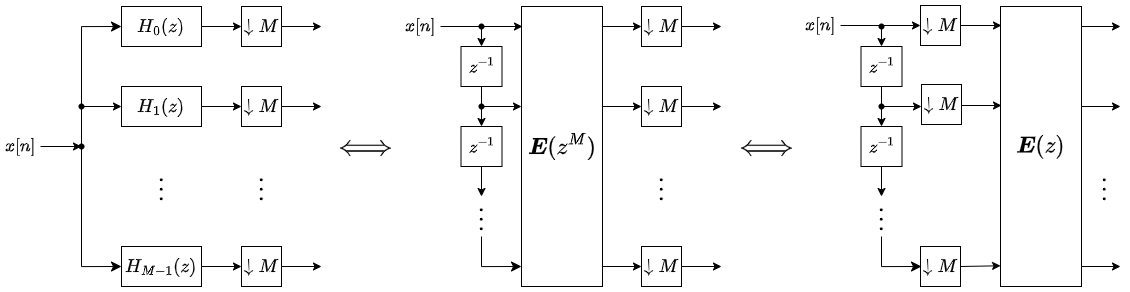
\includegraphics[width=115mm]{./figs/polyphase_representation_analyzer.drawio.png}
        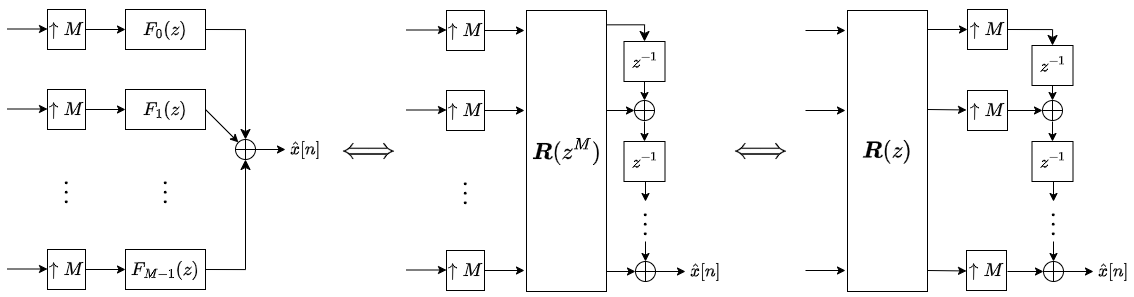
\includegraphics[width=115mm]{./figs/polyphase_representation_synthesizer.drawio.png}
    \end{figure}
\end{frame}

\begin{frame}[c]
    \frametitle{ポリフェーズ行列表現}
    $\ve{E}(z), \ve{R}(z)$により,$M$分割フィルタバンクは以下のように表せる
    \vspace{-13pt}
    \begin{figure}
        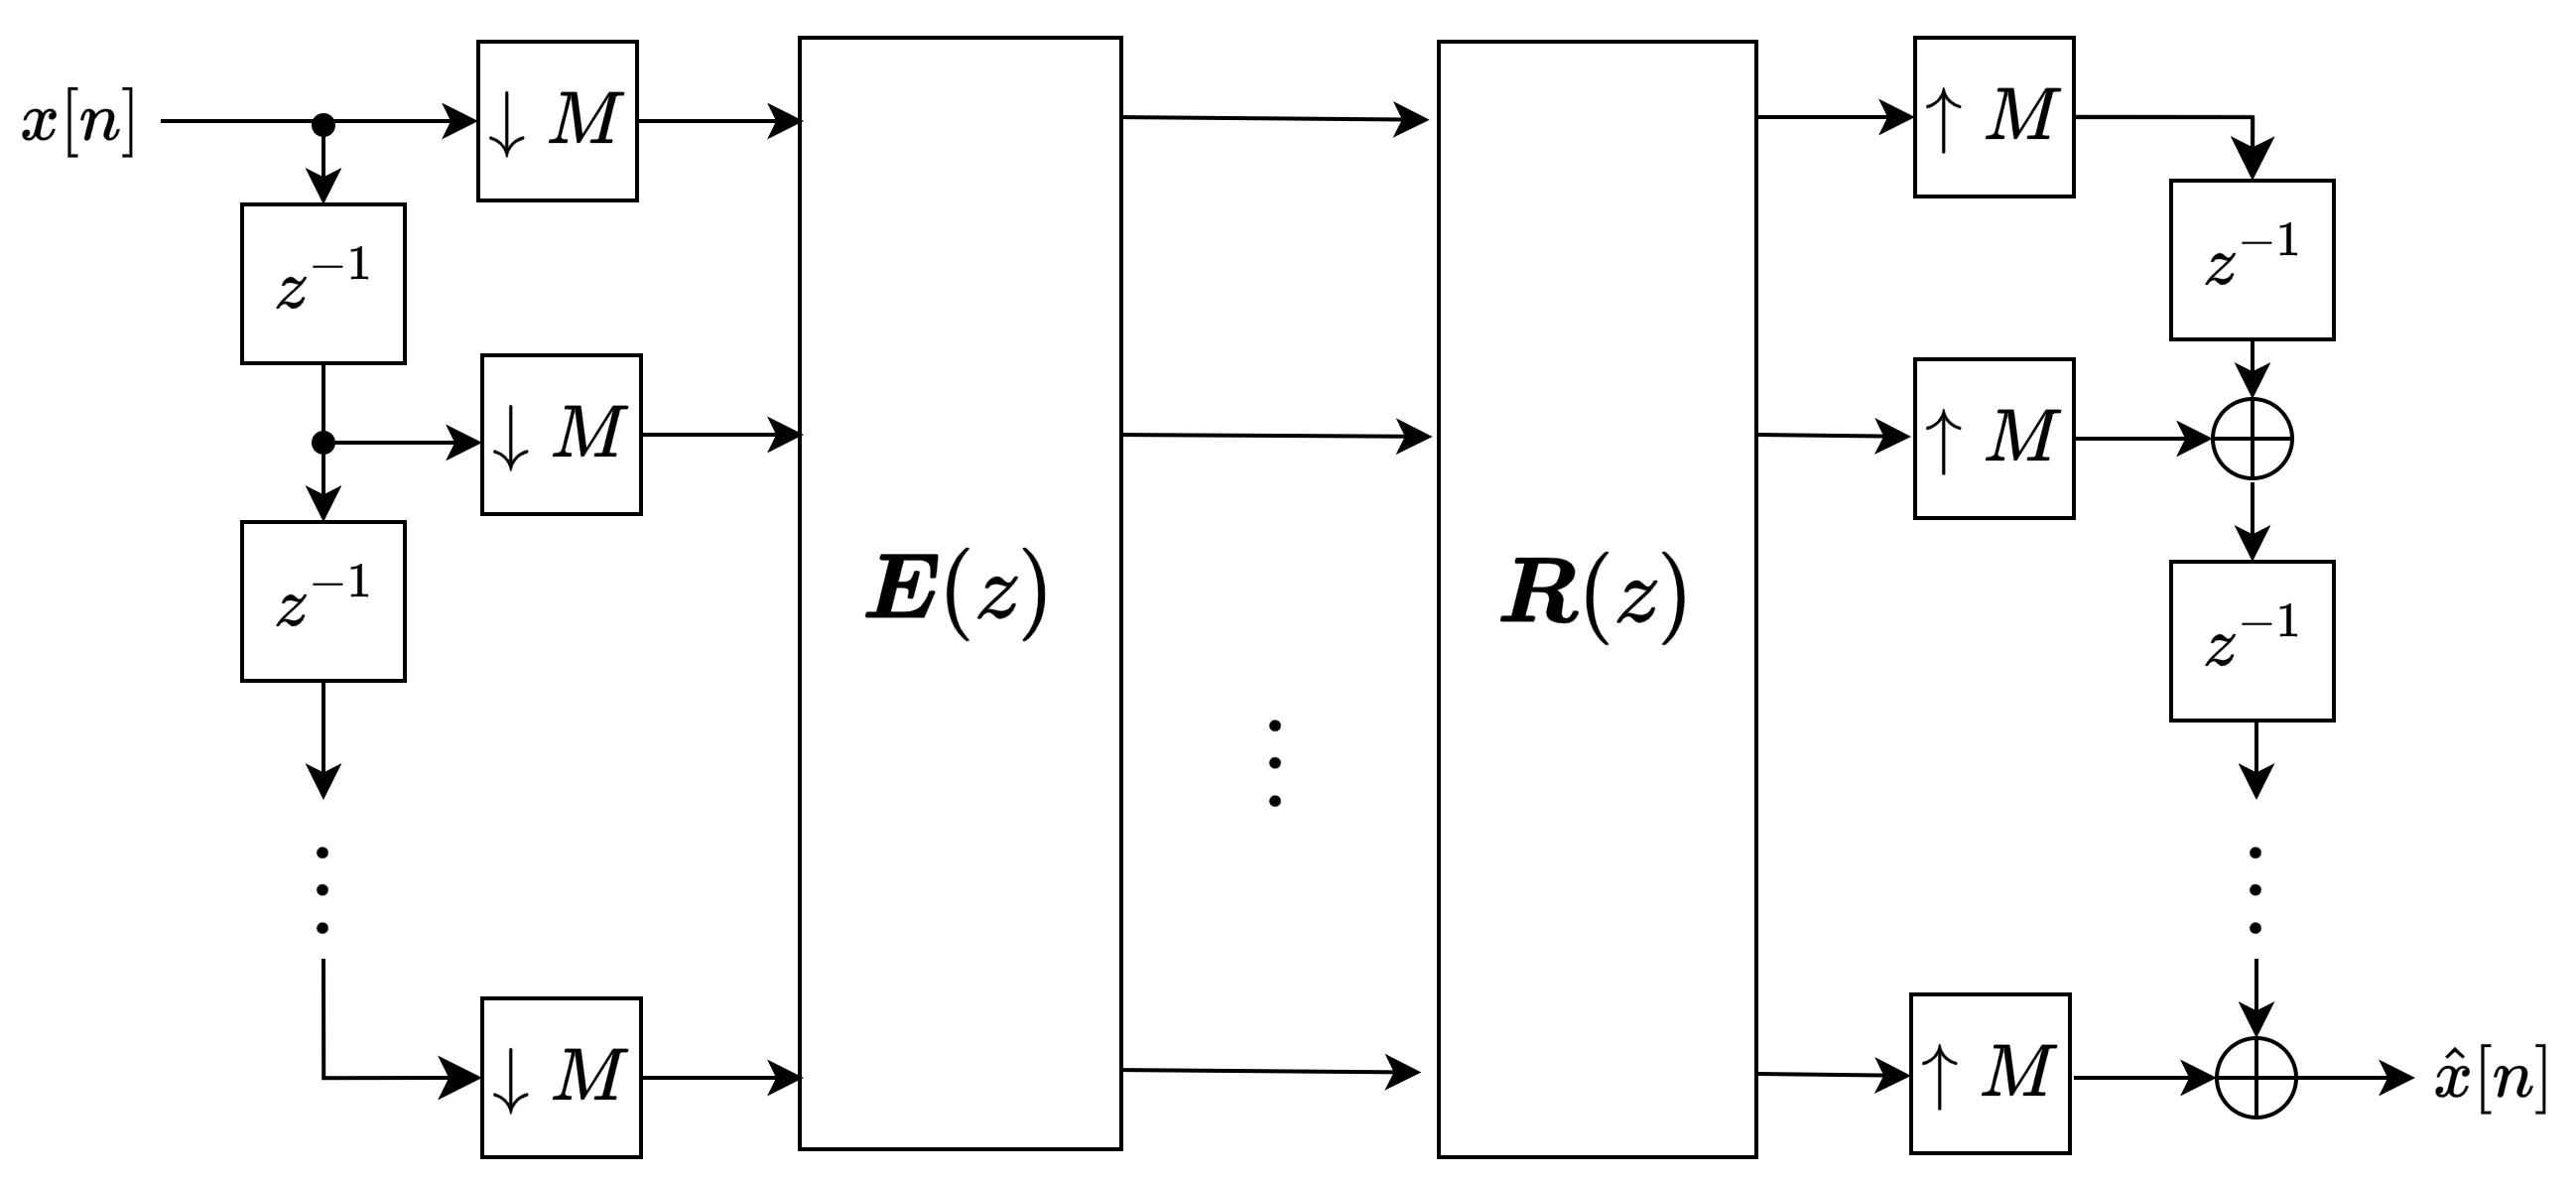
\includegraphics[width=120mm]{./figs/polyphase_representation_filter_bank.drawio.png}
    \end{figure}
\end{frame}

\begin{frame}[c]
    \frametitle{\scalebox{0.95}{完全再構成$M$分割フィルタバンク}}
    \begin{block}{}
        \vspace{-14pt}
        \begin{align}
            \ve{R}(z) \ve{E}(z) = a z^{-m_{0}} \ve{I} \quad (a \neq 0,\ m_{0} \in \mathbb{N}) \label{eq:filter_bank_PR_condition}
        \end{align}
        なら,$M$分割フィルタバンクは完全再構成\footnote{$\because$各バンドの遅延が$K$なら,$\hat{X}(z) = aM z^{-(M - 1 - K)}X(z)$}
    \end{block}
    \begin{figure}
        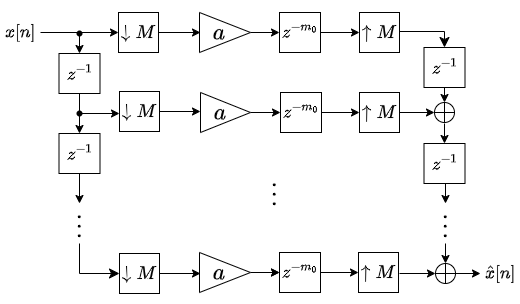
\includegraphics[width=70mm]{./figs/perfect_reconstraction_filter_bank.drawio.png}
    \end{figure}
\end{frame}

\begin{frame}[c]
    \frametitle{\scalebox{0.95}{完全再構成$M$分割フィルタバンク}}
    \eqref{eq:filter_bank_PR_condition}式より,$\ve{R}(z)$を
    \begin{align*}
        \ve{R}(z) = a z^{-m_{0}} \ve{E}(z)^{-1}
    \end{align*}
    とすれば完全再構成.しかし$\ve{E}(z)^{-1}$の計算が数値計算の安定性などの問題を孕む.
\end{frame}

\begin{frame}[c]
    \frametitle{\scalebox{0.95}{完全再構成$M$分割フィルタバンク}}
    $\ve{E}(z)^{-1}$の代わりに,$\ve{E}(z)$に\structure{パラユニタリ性}
    \begin{align}
        \widetilde{\ve{E}}(z) \ve{E}(z) = d \ve{I} \quad d \neq 0
    \end{align}
    を求める方法がある\footnote{$\widetilde{\ve{E}}(z) = \ve{E}_{\ast}(z^{-1})$で,下付きの$\ast$は係数の複素共役}.$\ve{E}(z)$がパラユニタリであれば,
    \begin{align*}
        \ve{R}(z) = a z^{-m_{0}} \widetilde{\ve{E}}(z)
    \end{align*}
    とすると完全再構成フィルタバンクになる.
\end{frame}

\begin{frame}[c]
    \frametitle{コサイン変調フィルタバンク}
    \begin{block}{コサイン変調フィルタバンク}
        \small
        \begin{align}
            h_{k}[n] &= 2 p_{0}[n] \cos \left[ \frac{\pi}{M} \left( k + \frac{1}{2} \right) \left( n - \frac{L - 1}{2} + \theta_{k} \right) \right] \\
            f_{k}[n] &= h_{k}[L - 1 - n] \label{eq:cos_modulated_synthesis_filter}
        \end{align}
        $p_{0}$:プロトタイプフィルタ,$M$:分割帯域数,$L$:タップ長,$\theta_{k} = (-1)^{k} \frac{\pi}{4}$
    \end{block}
\end{frame}

\begin{frame}[c]
    \frametitle{コサイン変調フィルタバンク}
    \begin{block}{}
    式\eqref{eq:cos_modulated_synthesis_filter}より,分析合成フィルタ$F_{k}(z)H_{k}(z)$は直線位相特性をもつ
    \end{block}
    \scriptsize
    (証明)
    \begin{align*}
        F_{k}(z) &= \sum_{n = -\infty}^{\infty} f_{k}[n] z^{-n} = \sum_{n = -\infty}^{\infty} h_{k}[L - 1 - n] z^{-n} = \sum_{n^{\prime} = -\infty}^{\infty} h_{k}[n^{\prime}] z^{-(L - 1 - n^{\prime})} \quad (n^{\prime} = L - 1 - n) \\
        &= z^{-(L-1)} \sum_{n^{\prime} = -\infty}^{\infty} h_{k}[n^{\prime}] z^{n^{\prime}} = z^{-(L-1)} H_{k}(z^{-1})
    \end{align*}
    $H_{k}(z)$の周波数特性を(極座標で)$H_{k}(\omega) = |H_{k}(\omega)| \exp[j \psi(\omega)]$と書くと,
    \begin{align*}
        F_{k}(\omega) &= \exp[-j(L - 1)\omega] H_{k}(-\omega) = \exp[-j(L - 1)\omega] |H_{k}(-\omega)| \exp[-j \psi(\omega)] \\
        &= \exp[-j(L - 1)\omega] |H_{k}(\omega)| \exp[-j \psi(\omega)] \quad \text{($\because$ 実係数FIRの振幅特性は偶)}
    \end{align*}
    だから,$F_{k}(\omega) H_{k}(\omega) = \exp[-j(L - 1)\omega] |H_{k}(\omega)|^{2}$となって直線位相特性をもつ.
\end{frame}

\begin{frame}[c]
    \frametitle{MP3のフィルタバンク}
    \begin{block}{MP3のフィルタバンク}
        \small
        \begin{align}
            y_{k}[t] &= \sum_{l = 0}^{511} x[t - l] h[l] \cos\left[ \frac{\pi}{32}\left( k + \frac{1}{2} \right) \left( l - 16 \right) \right] \\
            h[l] &= \left\{ \begin{array}{ll}
                -C_{l} & \lfloor l / 64 \rfloor \text{が偶数} \\
                 C_{l} & \lfloor l / 64 \rfloor \text{が奇数} \\
            \end{array} \right.
        \end{align}
        $C_{l}\ (l = 0,...,511)$は規格で設定
    \end{block}
    これは,$M = 32, L = 33$に該当
\end{frame}

\begin{frame}[c]
    \frametitle{MP3のフィルタバンク}
    プログラムでは,
    \begin{align*}
        y_{k}[t] &= \sum_{u = 0}^{7} \sum_{s = 0}^{63} x[t - s - 64u] C_{s + 64u} t_{k,s} \\
        t_{k,s} &:= \cos\left[ \frac{\pi}{32}\left( k + \frac{1}{2} \right) \left( s - 16 \right) \right]
    \end{align*}
    で計算している.この式が定義式通りであることを示す.
\end{frame}

\begin{frame}[c]
    \frametitle{MP3のフィルタバンク}
    \scriptsize
    \begin{align}
        y_{k}[t] &= \sum_{l = 0}^{511} x[t - l] h[l] t_{k,l} = \sum_{u = 0}^{7} \sum_{s = 0}^{63} x[t - s - 64u] h[s + 64u] t_{k,s+64u} \nonumber \\
        &= \sum_{u = 0}^{7} \sum_{s = 0}^{63} x[t - s - 64u] (-1)^{u} C_{s + 64u} t_{k,s+64u} \label{eq:mp3_filterbank_progaram_deviation}
    \end{align}
    ここで,
    \begin{align*}
        t_{k,s+64u} &= \cos\left[ \frac{\pi}{32} \left( k + \frac{1}{2} \right) (s + 64u - 16) \right] = \cos\left[ \frac{\pi}{32} \left( k + \frac{1}{2} \right) (s - 16) + \pi \left( 2k + 1 \right) u \right] \\
        &= \cos\left[ \frac{\pi}{32} \left( k + \frac{1}{2} \right) (s - 16) \right]\cos\left[ \pi(2k + 1)u \right] \\
        &\quad - \sin\left[ \frac{\pi}{32} \left( k + \frac{1}{2} \right) (s - 16) \right]\sin\left[ \pi(2k + 1)u \right]
        % &= (-1)^{u} \cos\left[ \frac{\pi}{32} \left( k + \frac{1}{2} \right) (s - 16) \right] = (-1)^{u} 
        = (-1)^{u} t_{k,s}
    \end{align*}
    だから,これを式\eqref{eq:mp3_filterbank_progaram_deviation}に代入すれば欲しい結果が得られる.
\end{frame}

\begin{frame}[c]
    \frametitle{電力相補条件の確認}
    \scriptsize
    MP3のフィルタバンクでは
    \begin{align*}
        G_{l}(z) &= \sum_{n = -\infty}^{\infty} h[2nM + l] z^{-n} = \sum_{n = 0}^{7} h[64n + l] z^{-n} = \sum_{n = 0}^{7} (-1)^{n} C_{64 + l} z^{-n} \\
        G_{M+l}(z) &= \sum_{n = 0}^{7} h[64n + 32 + l] z^{-n} = \sum_{n = 0}^{7} (-1)^{n} C_{64n + 32 + l} z^{-n} \\
        G_{l}(z^{-1}) &= \sum_{n = -\infty}^{\infty} h[64n + l] (z^{-1})^{-n} = \sum_{n = -\infty}^{\infty} h[-64n + l] z^{-n} = \sum_{n = -7}^{0} (-1)^{n} C_{-64n + l} z^{-n} \\
        G_{M+l}(z^{-1}) &= \sum_{n = 0}^{7} h[-64n + 32 + l] z^{-n} = \sum_{n = 0}^{7} (-1)^{n} C_{-64n + 32 + l} z^{-n} \\
    \end{align*}
    となる.
\end{frame}

\subsection{MDCT}

\begin{frame}[c]
    \frametitle{MDCT}
\end{frame}

\subsection{エイリアス削除バタフライ演算}

\begin{frame}[c]
    \frametitle{エイリアス削除バタフライ演算}
\end{frame}

\section{量子化}

\begin{frame}[c]
    \frametitle{非線形量子化}
\end{frame}

\section{符号化}

\begin{frame}[c]
    \frametitle{ハフマン符号}
\end{frame}

\section{聴覚モデル}

\begin{frame}[c]
    \frametitle{聴覚モデル}
\end{frame}

\end{document}
